%% 10. Parallel Primitives

% Reductions

\begin{frame}{Parallel Primitives}

\begin{block}{Reductions}
  \begin{itemize}
   \item Use $N$ values to compute $1$ result value
   \item Examples: Dot-products, vector norms, etc.
  \end{itemize}
\end{block}

\begin{block}{Reductions with Few Threads}
  \begin{itemize}
   \item Decompose $N$ into chunks for each thread
   \item Compute chunks in parallel
   \item Merge results with single thread
  \end{itemize}
\end{block}

\begin{center} 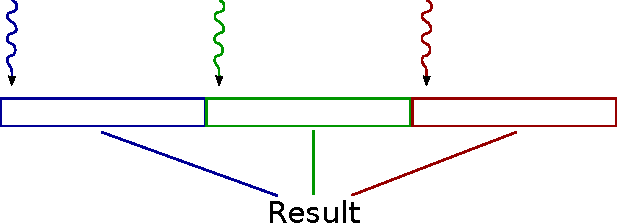
\includegraphics[width=0.7\textwidth]{figures/reductions-thread} \end{center}

\end{frame}





\begin{frame}{Parallel Primitives}

\begin{block}{Reductions with Many Threads}
  \begin{itemize}
   \item Decompose $N$ into chunks for each workgroup
   \item Use fast on-chip synchronization within each workgroup
   \item Sum result for each workgroup separately
  \end{itemize}
\end{block}

\begin{center} 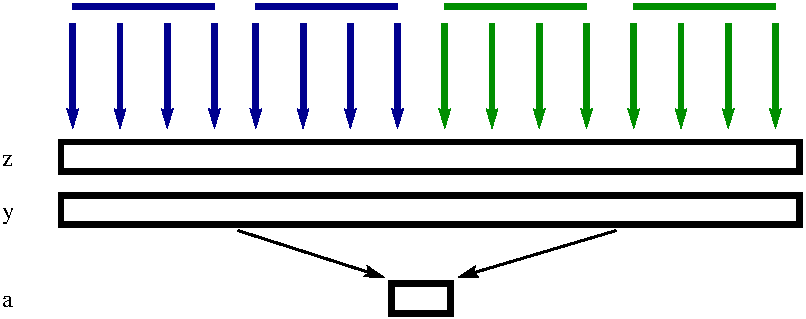
\includegraphics[width=0.8\textwidth]{figures/inner-product-kernel} \end{center}


\end{frame}




% \begin{frame}[fragile]{Parallel Primitives}
% 
%  \begin{block}{Reductions with Many Threads}
%   \begin{center} 
%    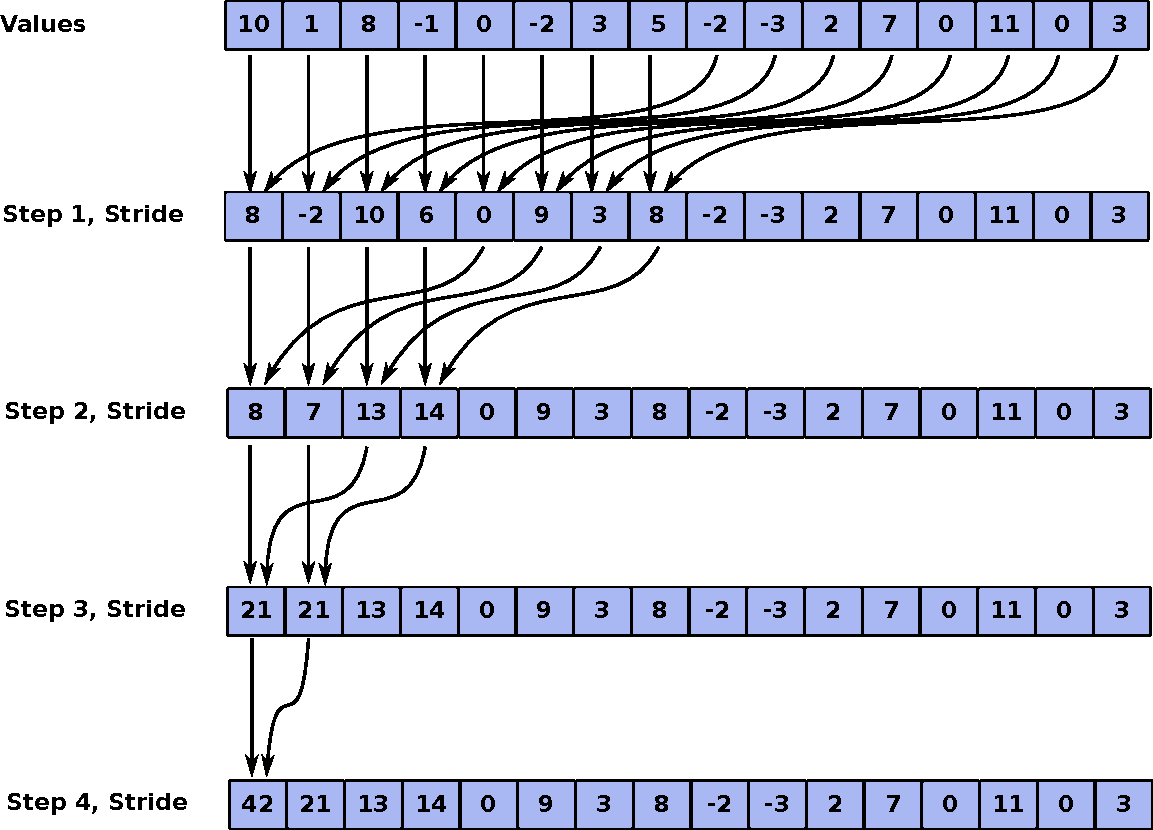
\includegraphics[width=0.6\textwidth]{figures/reduction}
%   \end{center}
%   \vspace*{2.45cm}
%  \end{block}
% \end{frame}

%%

\begin{frame}[fragile]{Parallel Primitives}

\begin{block}{Reductions with Many Threads}
\begin{center} 
  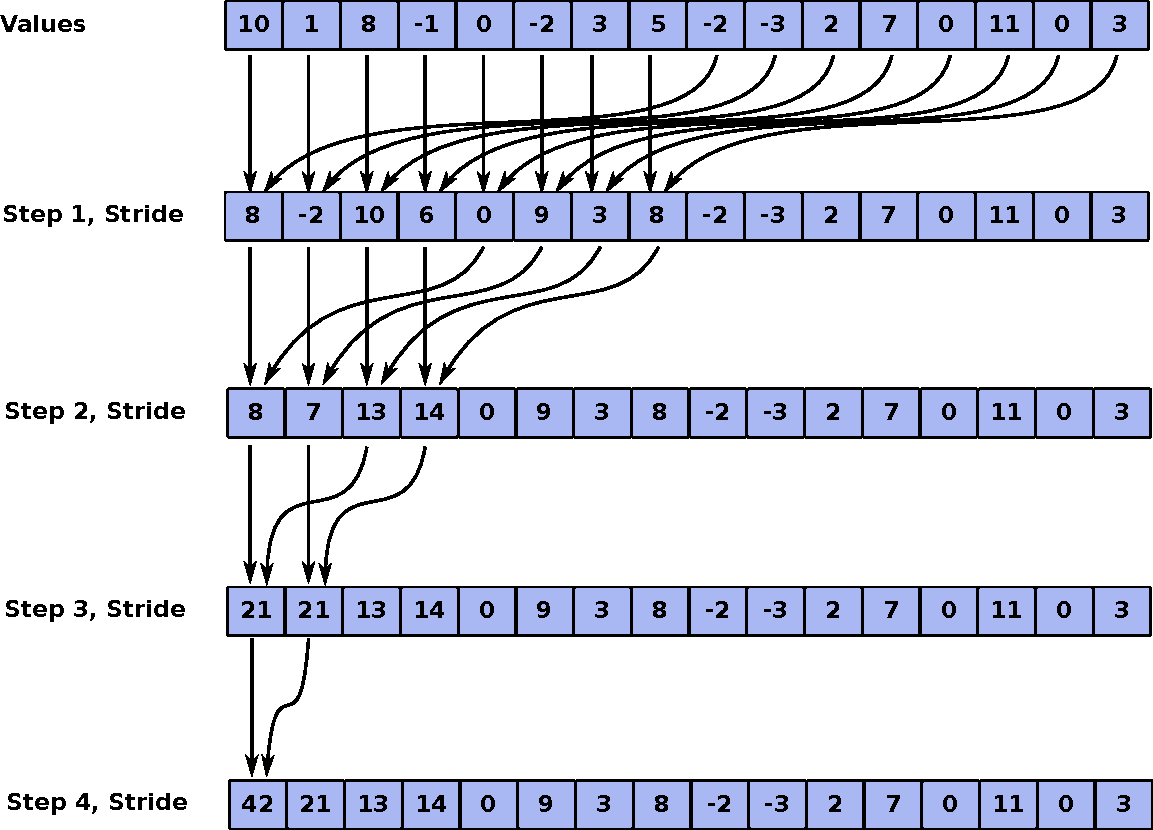
\includegraphics[width=0.6\textwidth]{figures/reduction}
\end{center}
\vspace*{-0.5cm}
\end{block}
\begin{center}
\begin{lstlisting}
shared_m[threadIdx.x] = thread_sum;
for (int stride = blockDim.x/2; stride>0; stride/=2) {
  __syncthreads();
  if (threadIdx.x < stride)
    shared_m[threadIdx.x] += shared_m[threadIdx.x+stride];
}
\end{lstlisting}
\end{center}

\end{frame}



%%%%%%%%%%%%% Load and FLOPs: Use shared memory





%%%%%%%%%%%% Prefix sum: Explain why and how it works. Use FEM as example

\begin{frame}[fragile]{Parallel Primitives}

\begin{minipage}{0.7\textwidth}
\begin{block}{Prefix Sum}
  \begin{itemize}
   \item Inclusive: Determine $y_i = \sum_{k=1}^i x_k$
   \item Exclusive: Determine $y_i = \sum_{k=1}^{i-1} x_k$, $y_1 = 0$
  \end{itemize}
\end{block}

%\pause
\begin{block}{Example}
 \begin{itemize}
  \item x: $4$, $3$,  $\hphantom{1}6$,  $\hphantom{1}5$,  $\hphantom{1}4$,  $\hphantom{1}7$,  $\hphantom{1}4$,  $\hphantom{1}4$,  $\hphantom{1}4$
  \item y: $4$, $7$,             $13$,             $18$,             $22$,             $29$,             $33$,             $37$,             $41$ (inclusive)
  \item y: $0$, $4$,  $\hphantom{1}7$,             $13$,             $18$,             $22$,             $29$,             $33$,             $37$ (exclusive)
 \end{itemize}

\end{block}

\begin{block}{Applications}
  \begin{itemize}
   \item Sparse matrix setup
   \item Graph algorithms
  \end{itemize}
\end{block}
\vspace*{1cm}
\end{minipage}
\begin{minipage}{0.2\textwidth}
\vspace*{4cm} \hspace*{-3.5cm}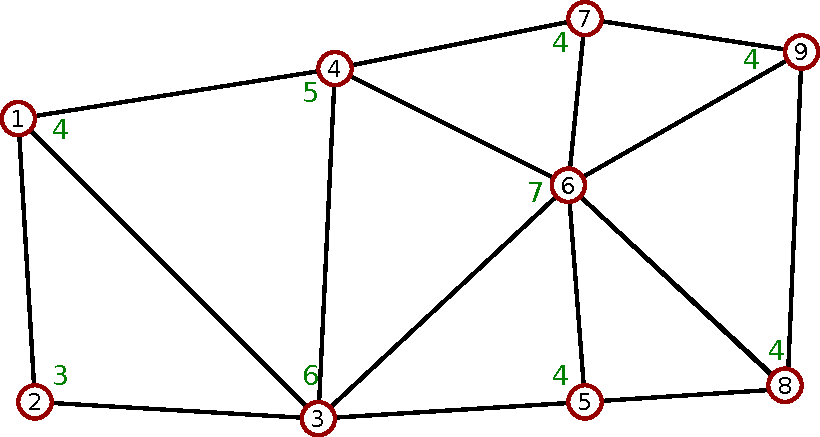
\includegraphics[width=2.8\textwidth]{figures/graph-1}
\end{minipage}

\end{frame}


%%


\begin{frame}[fragile]{Parallel Primitives}

 \begin{block}{Prefix Sum Implementation}
  \begin{center} 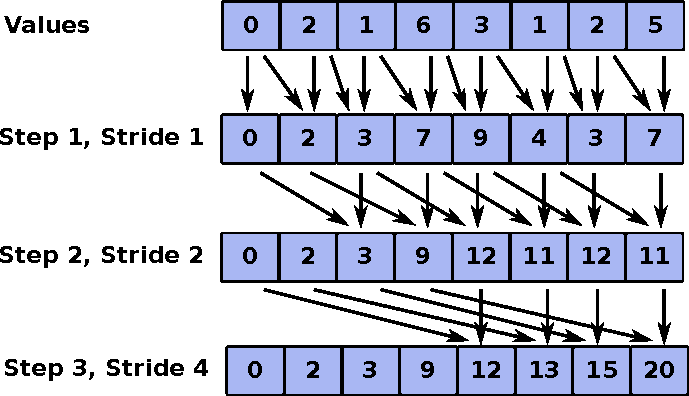
\includegraphics[width=0.5\textwidth]{figures/prefixsum} \end{center}
  \begin{lstlisting}
for(int stride = 1; stride < blockDim.x; stride *= 2)
{
  __syncthreads();
  shared_buffer[threadIdx.x] = my_value;
  __syncthreads();
  if (threadIdx.x >= stride)
    my_value += shared_buffer[threadIdx.x - stride];
}
__syncthreads();
shared_buffer[threadIdx.x] = my_value;
  \end{lstlisting}
 \end{block}
\end{frame}





%%
%%%%%%%%%%%% Coloring: Rework ILU example, mention limitations
%%






\begin{frame}[fragile]
\frametitle{Parallel Primitives}

  \begin{minipage}{0.5\textwidth}
    \begin{block}{ILU - Basic Idea}
      \begin{itemize}
        \item Factor sparse matrix $\matrix A \approx \tilde{\matrix L} \tilde{\matrix U}$
        \item $\tilde{\matrix L}$ and $\tilde{\matrix U}$ sparse, triangular
        \item ILU0: Pattern of $\tilde{\matrix L}$, $\tilde{\matrix U}$ equal to $\matrix A$
        \item ILUT: Keep $k$ elements per row
      \end{itemize}
    \end{block}
  \end{minipage}
%
  \begin{minipage}{0.45\textwidth}
    \begin{block}{Solver Cycle Phase}
      \vspace*{-0.1cm}
      \begin{itemize}
        \item Residual correction ${\color{red}\tilde{\matrix L}} \tilde{\matrix U} x = z$
        \item Forward solve ${\color{red}\tilde{\matrix L}} y = z$
        \item Backward solve $\tilde{\matrix U} x = y$
        \item Little parallelism in general
      \end{itemize}
    \end{block}
  \end{minipage}


  \begin{align*} 
   \left(
   \begin{array}{ccccccccc}
     \textstyle 5 &  \textstyle \times & \textstyle \times     & \textstyle \times  &   & \textstyle \times     & \textstyle \times &   &   \\
     \textstyle \color{red} \times & \textstyle 3 & \textstyle \times      &    &   &      &   &  &   \\
    \textstyle \color{red} \times & \textstyle \color{red} \times & \textstyle 4     & \textstyle \times  &   &       &   &   &   \\
%
    \textstyle \color{red} \times &   &  \textstyle\color{red}  \times     & \textstyle 5  & \textstyle \times & \textstyle \times     &   &   & \textstyle \times \\
      &   &       & \textstyle \color{red} \times  & \textstyle 5 & \textstyle \times     &   & \textstyle \times & \textstyle \times \\
    \textstyle \color{red} \times &   &      & \textstyle \color{red} \times  & \textstyle \color{red} \times & \textstyle 6     & \textstyle \times & \textstyle \times &  \\
%
    \textstyle \color{red} \times &  &       &    &   & \textstyle\color{red}  \times     & \textstyle 3 &   &   \\
      &   &       &    & \textstyle\color{red}  \times & \textstyle \color{red} \times    &   & \textstyle 4 & \textstyle \times \\
      &   &      & \textstyle\color{red}  \times  & \textstyle \color{red} \times &      &   & \textstyle \color{red} \times & \textstyle 4 \\
   \end{array}
         \right)
  \end{align*}

 
\end{frame}





\begin{frame}[fragile]
\frametitle{Parallel Primitives}

     \begin{block}{ILU Level Scheduling}
      \begin{itemize}
        \item Build dependency graph
        \item Substitute as many entries as possible simultaneously
        \item Trade-off: Each step vs. multiple steps in a single kernel
      \end{itemize}

      \begin{center}
%     \only<1>{ 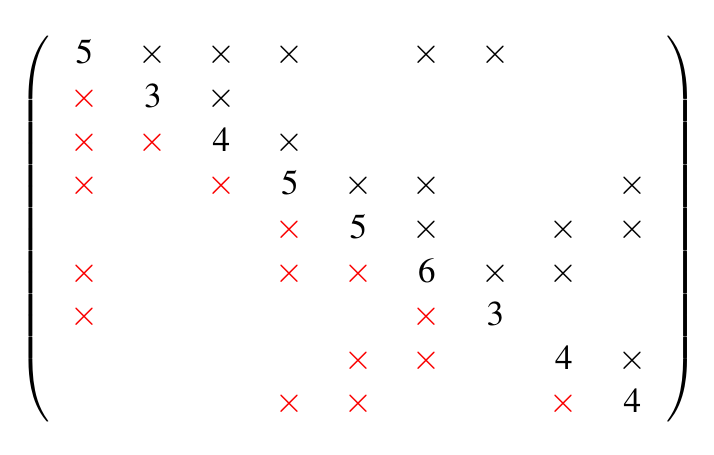
\includegraphics[width=0.65\textwidth]{figures/level-scheduling.png} }
%     \only<2>{ 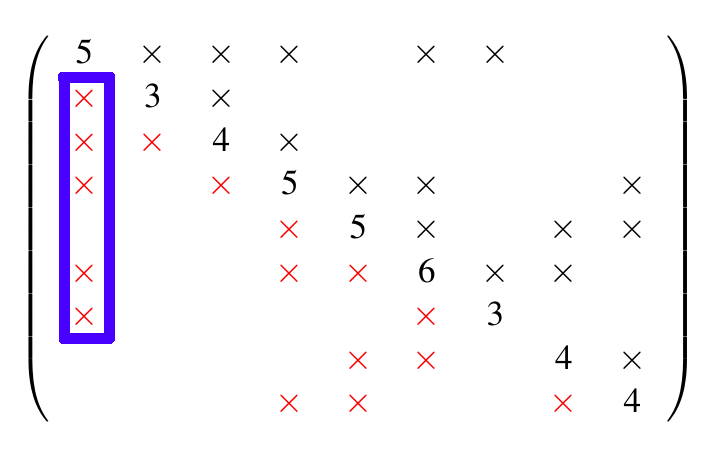
\includegraphics[width=0.65\textwidth]{figures/level-scheduling-1.png} }
%     \only<3>{ 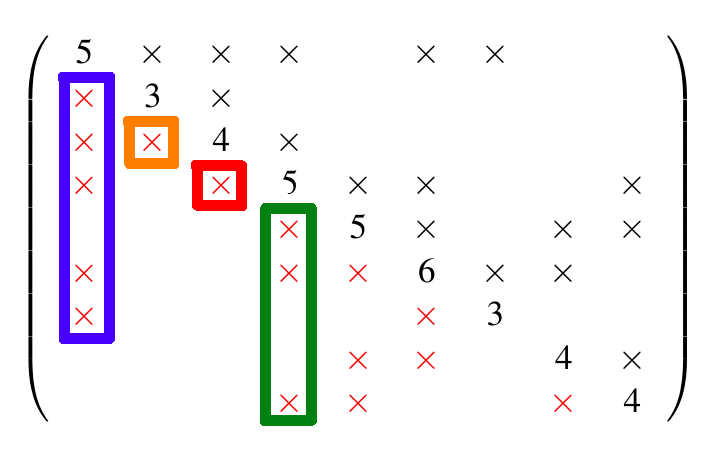
\includegraphics[width=0.65\textwidth]{figures/level-scheduling-3.png} }
       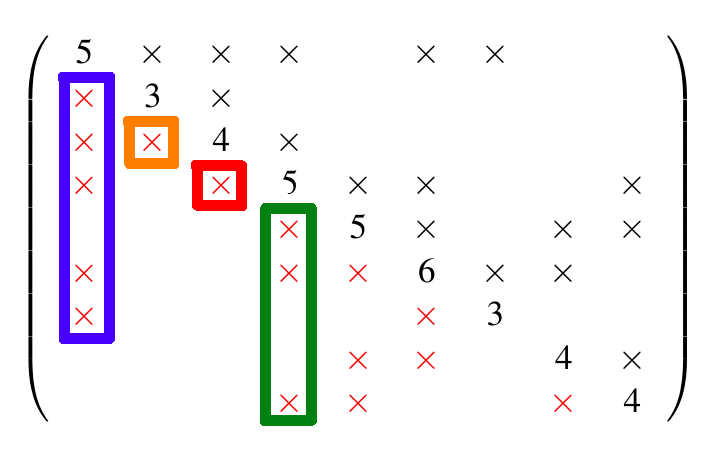
\includegraphics[width=0.65\textwidth]{figures/level-scheduling-3.png}
      \end{center}

    \end{block}
\end{frame}


\begin{frame}[fragile]
\frametitle{Parallel Primitives}

     \begin{block}{ILU Interpretation on Structured Grids}
      \begin{itemize}
        \item 2d finite-difference discretization
        \item Substitution whenever all neighbors with smaller index computed
        \item Works particularly well in 3d
      \end{itemize}

      \begin{center}
%     \only<1>{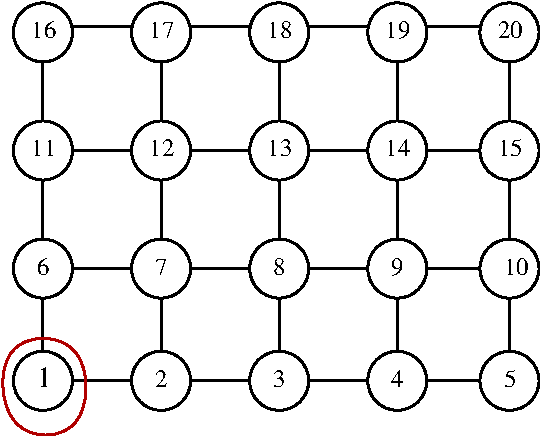
\includegraphics[width=0.4\textwidth]{figures/2d-grid-1}\hspace*{1.0cm}
\includegraphics[width=0.4\textwidth]{figures/order_lexi}}
%     \only<2>{\hspace*{-0.085cm}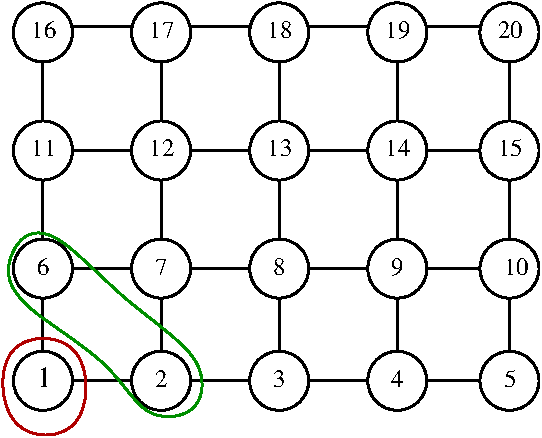
\includegraphics[width=0.4\textwidth]{figures/2d-grid-2}\hspace*{1.0cm}
\includegraphics[width=0.4\textwidth]{figures/order_lexi}}
    \only<1>{\hspace*{-0.17cm}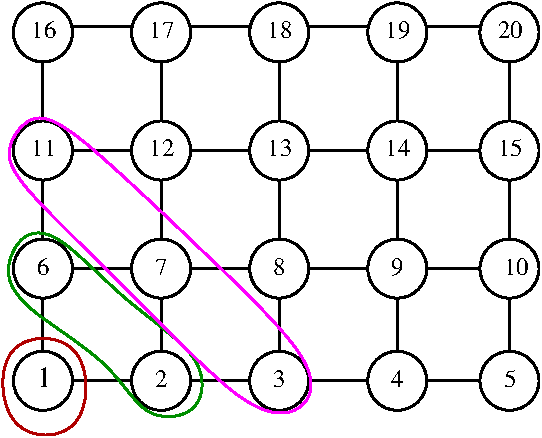
\includegraphics[width=0.4\textwidth]{figures/2d-grid-3}\hspace*{1.0cm}
\includegraphics[width=0.4\textwidth]{figures/order_lexi}}
%
%     \only<4>{\hspace*{-0.255cm}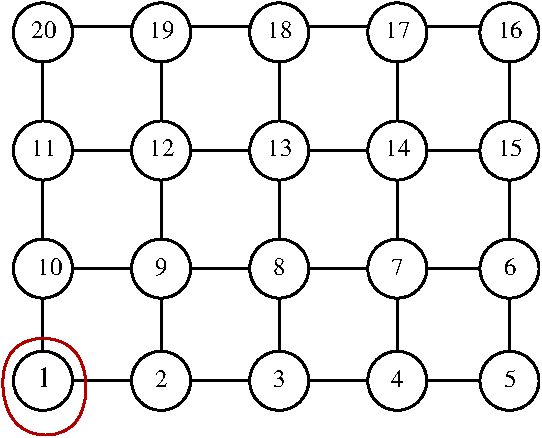
\includegraphics[width=0.4\textwidth]{figures/2d-grid-1-bad}\hspace*{1.0cm}
\includegraphics[width=0.4\textwidth]{figures/order_bad}}
%     \only<5>{\hspace*{-0.34cm}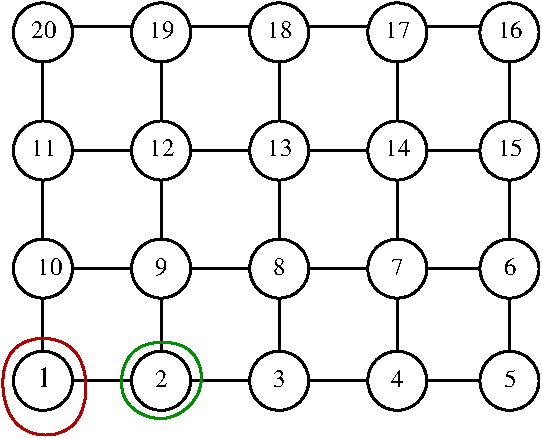
\includegraphics[width=0.4\textwidth]{figures/2d-grid-2-bad}\hspace*{1.0cm}
\includegraphics[width=0.4\textwidth]{figures/order_bad}}
    \only<2>{\hspace*{-0.425cm}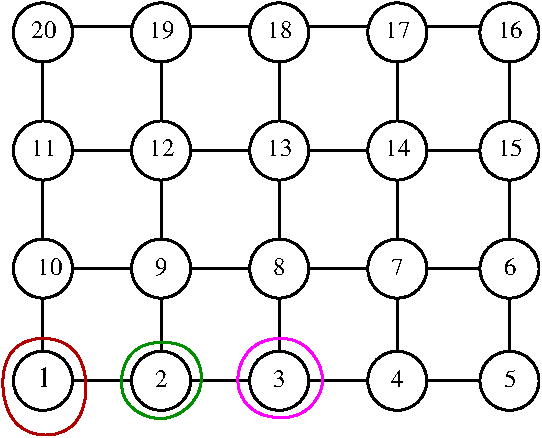
\includegraphics[width=0.4\textwidth]{figures/2d-grid-3-bad}\hspace*{1.0cm}
\includegraphics[width=0.4\textwidth]{figures/order_bad}}
%
%     \only<7>{\hspace*{-0.51cm}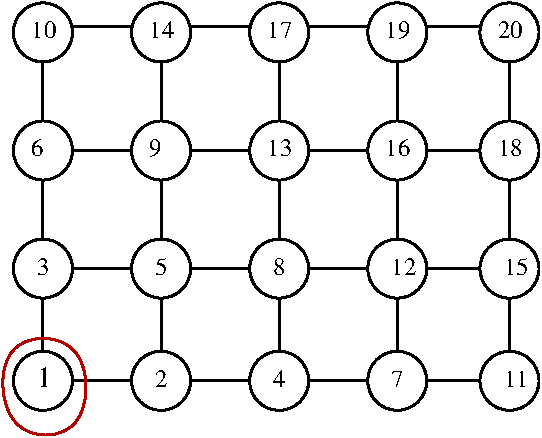
\includegraphics[width=0.4\textwidth]{figures/2d-grid-1-min}\hspace*{1.0cm}
\includegraphics[width=0.4\textwidth]{figures/order_min}}
%     \only<8>{\hspace*{-0.595cm}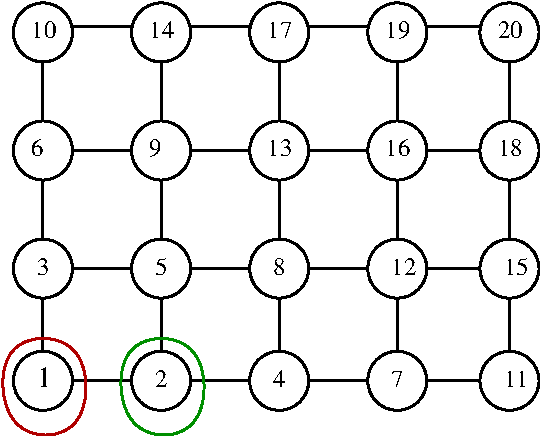
\includegraphics[width=0.4\textwidth]{figures/2d-grid-2-min}\hspace*{1.0cm}
\includegraphics[width=0.4\textwidth]{figures/order_min}}
    \only<3>{\hspace*{-0.68cm}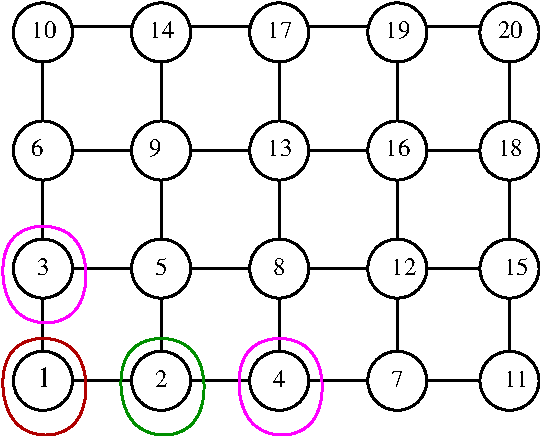
\includegraphics[width=0.4\textwidth]{figures/2d-grid-3-min}\hspace*{1.0cm}
\includegraphics[width=0.4\textwidth]{figures/order_min}}
%
%     \only<10>{\hspace*{-0.765cm}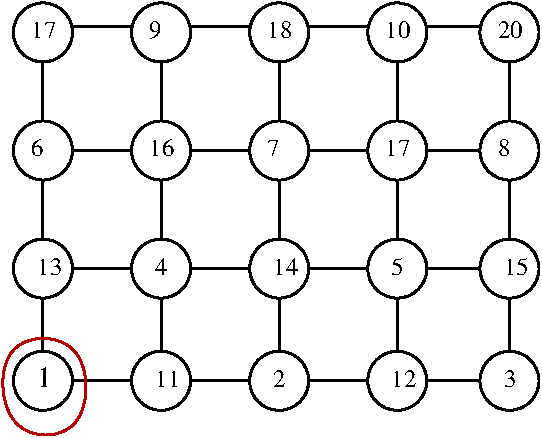
\includegraphics[width=0.4\textwidth]{figures/2d-grid-1-rb}\hspace*{1.0cm}
\includegraphics[width=0.4\textwidth]{figures/order_rb}}
%     \only<11>{\hspace*{-0.75cm}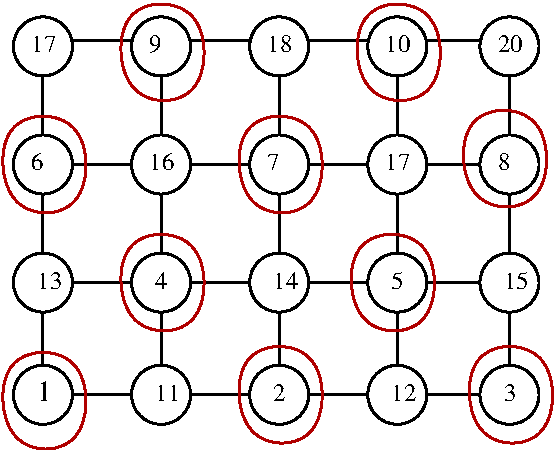
\includegraphics[width=0.41\textwidth]{figures/2d-grid-2-rb}\hspace*{0.9cm}
\includegraphics[width=0.4\textwidth]{figures/order_rb}}
    \only<4>{\hspace*{-0.75cm}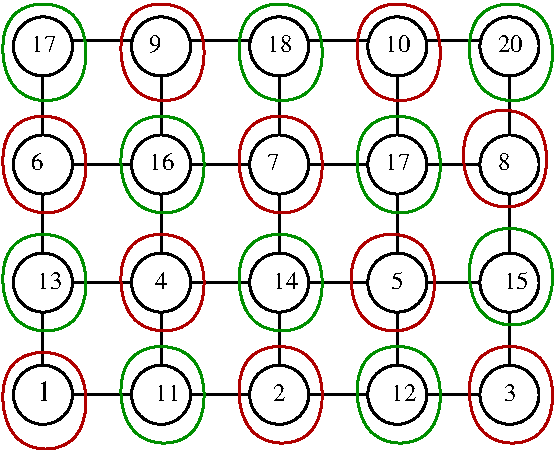
\includegraphics[width=0.41\textwidth]{figures/2d-grid-3-rb}\hspace*{0.9cm}
\includegraphics[width=0.4\textwidth]{figures/order_rb}}
      \end{center}

    \end{block}
\end{frame}






%%
%%%%%%%%%%%% Libraries
%%


\begin{frame}[fragile]
\frametitle{Parallel Primitives}

 \begin{block}{Other Parallel Primitives}
  \begin{itemize}
   \item Sort
   \item Gather and Scatter
   \item Load to shared memory and work there
   \item etc.
  \end{itemize}
 \end{block}

 \begin{block}{GPU-Accelerated Software Libraries}
  \begin{itemize}
   \item Linear Algebra: ViennaCL, MAGMA, CUSP, VexCL, ...
   \item Solvers: ViennaCL, MAGMA, cuSolver, Paralution, clAMG, ...
   \item FFT: cuFFT, clFFT, FFTW, ...
   \item Primitives: VexCL, Boost.Compute, ...
   \item Machine Learning: Caffe, cuDNN, ...
  \end{itemize}
 \end{block}

\end{frame}

